% Canonical float definitions; invoked beside their Results paragraphs.
\newcommand{\MainFigureOne}{%
\begin{figure}[!htb]\centering
% Retain the original vector panel a (top 142 bp); place the approved new panel b below.
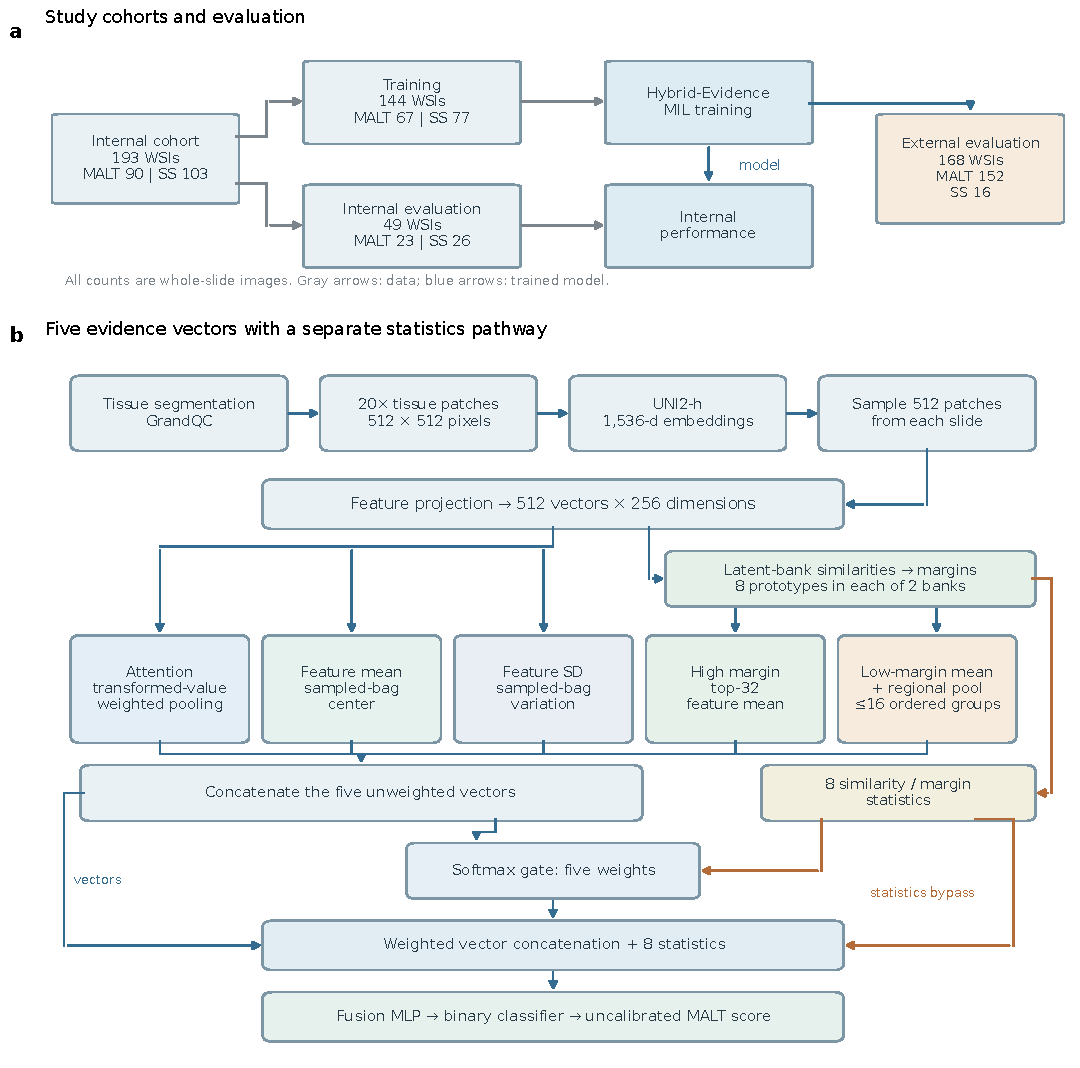
\includegraphics[width=\textwidth,trim=0 370.663757bp 0 0,clip]{figures/Figure_1_study_framework.pdf}\par\vspace{4pt}
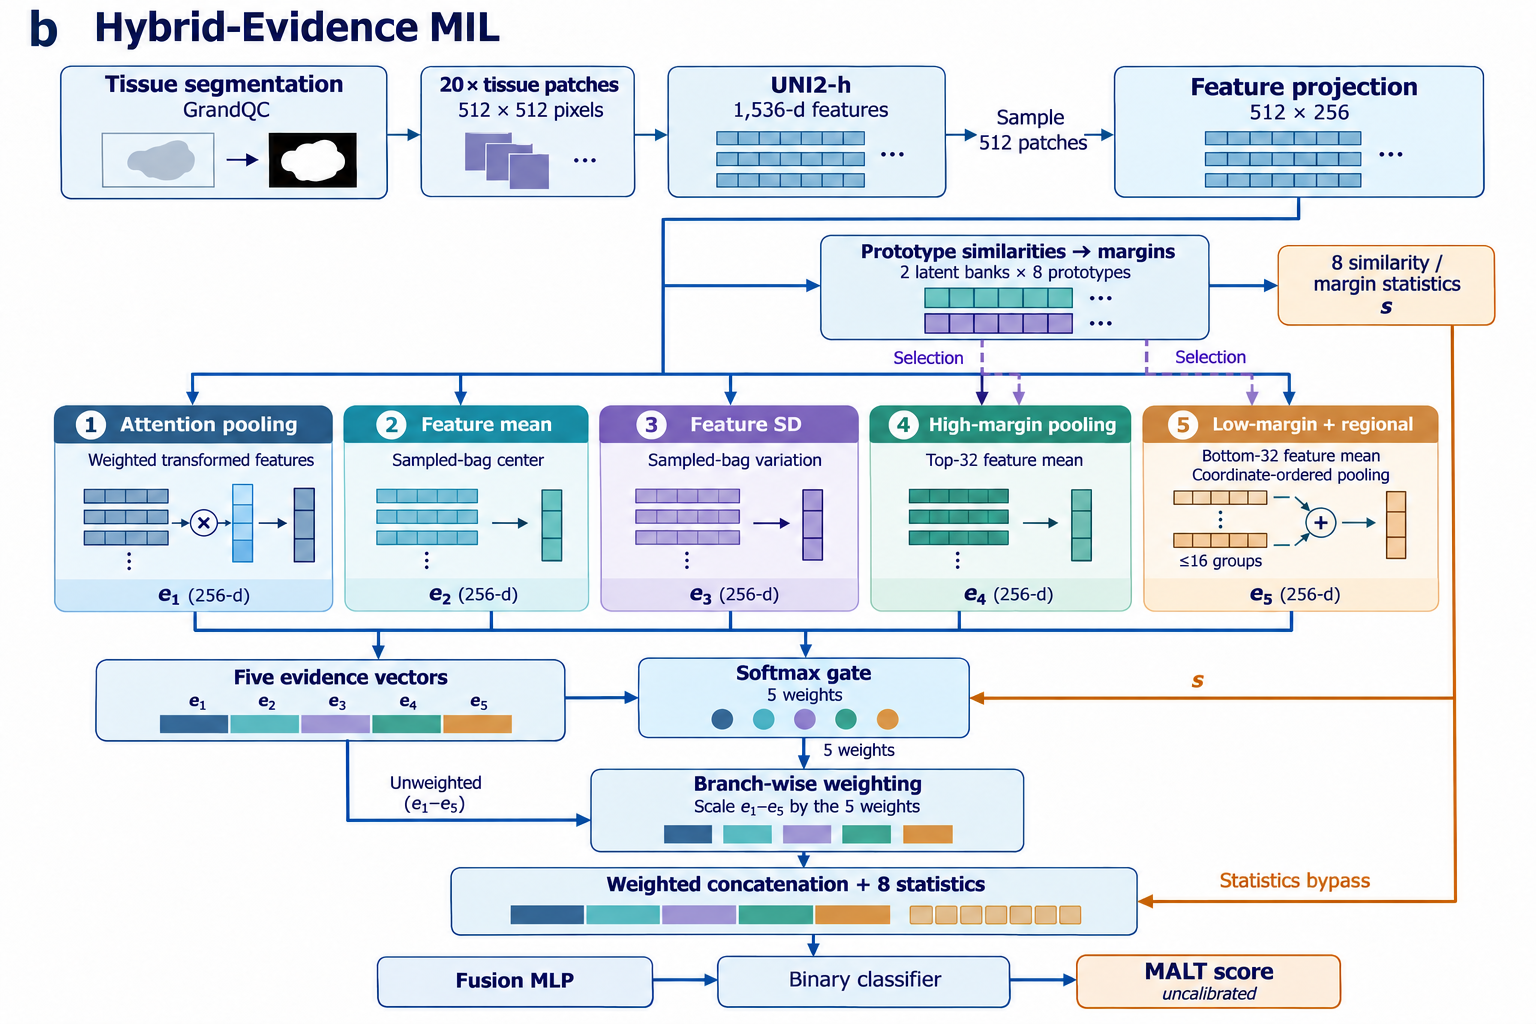
\includegraphics[width=\textwidth]{figures/Figure_1b_model_ai.png}
\caption{\textbf{Study cohorts and multi-evidence classification}. \textbf{a,} Internal training and validation cohorts and the external evaluation material; all counts are WSIs. The internal validation slides also selected checkpoints; patient-level separation remains unverified. Gray arrows indicate data and blue arrows indicate the trained model. \textbf{b,} Projected UNI2-h features form five evidence vectors. Similarities to two latent prototype banks and their margins generate instance selections and eight separate statistics. The low-margin instance and regional vectors are added; regional tokens are formed by coordinate-ordered grouping and pooled without explicit interregional spatial relations. Gate weights scale the five vectors before concatenation; the statistics also enter fusion through an unweighted pathway. Source data are provided in internal\_cohort.csv and external\_final\_predictions.csv.}\label{fig:1}
\end{figure}
}

\newcommand{\MainFigureTwo}{%
\begin{figure}[!htb]\centering
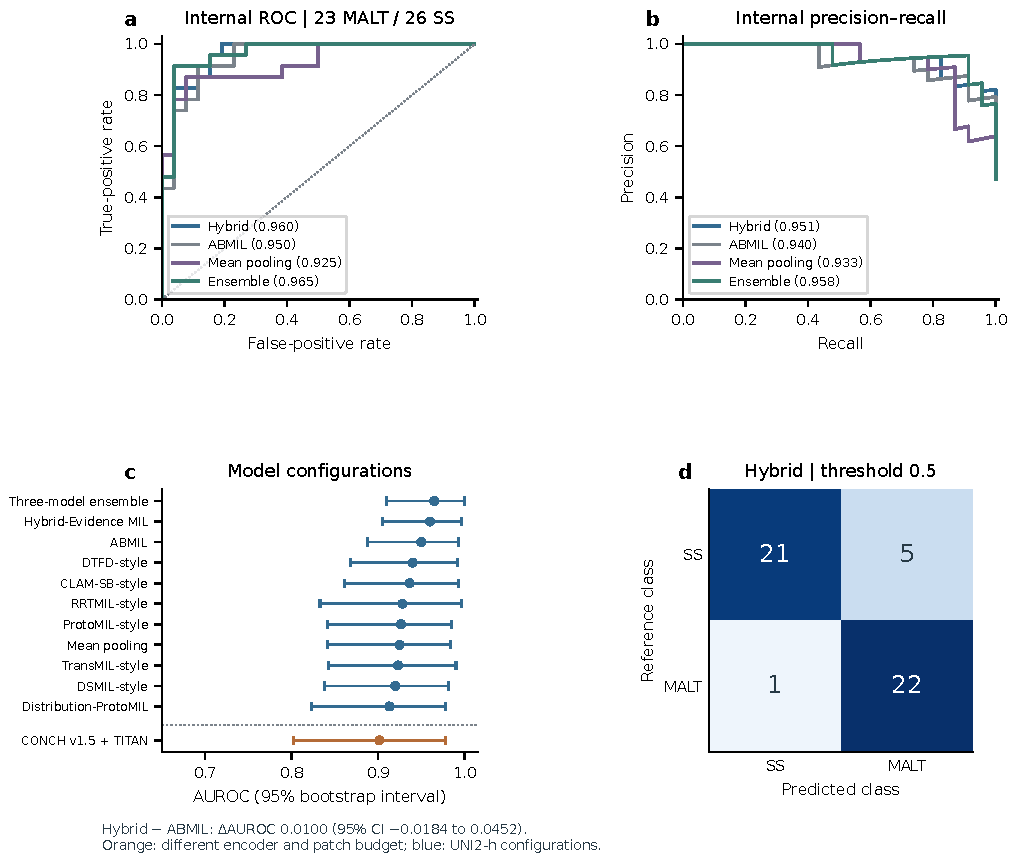
\includegraphics[width=\textwidth,height=.76\textheight,keepaspectratio]{figures/Figure_2_internal_performance.pdf}
\caption{\textbf{Internal validation discrimination and model configurations}. \textbf{a,b,} ROC and precision--recall curves on 49 WSIs (23 MALT and 26 SS). \textbf{c,} AUROC and 95\% intervals from 2,000 label-stratified WSI bootstrap samples of fixed predictions. Blue points use UNI2-h; the orange point uses a different encoder and patch budget. Simplified implementations retain their ``-style'' labels. The comparisons include complete implementations with different projection dimensions and training budgets. \textbf{d,} Hybrid confusion matrix at threshold 0.5. The 49 slides also selected checkpoints; intervals condition on fixed predictions and omit selection uncertainty. The paired Hybrid--ABMIL difference interval crosses zero. Source data are provided in internal\_model\_metrics.csv, paired\_model\_comparisons.csv and model-specific prediction tables.}\label{fig:2}
\end{figure}
}

\newcommand{\MainFigureThree}{%
\begin{figure}[!htb]\centering
\fbox{\begin{minipage}[c][35mm][c]{.88\textwidth}\centering
\textbf{Omitted from this public repository copy}\\[6pt]
This figure contains tissue images or individual-slide observations.\\
The complete figure is retained in the local manuscript archive.
\end{minipage}}
\caption{\textbf{External performance and archive-tag composition}. \textbf{a,b,} ROC and precision--recall curves for four frozen model checkpoints on the same 168 WSIs (152 MALT and 16 SS), using identical reference bags for each slide. Legend values indicate AUROC and average precision, respectively. These compare complete implementations. The dotted PR reference is the MALT fraction. \textbf{c,} Confusion matrix at threshold 0.5. \textbf{d,} Individual uncalibrated model scores by diagnostic group and archive stain tag. Counts indicate correct predictions divided by group size; black marks show medians. Jitter separates points only. H\&E-like, IHC/special and HE-archive labels are provisional archive descriptors, not pathology-confirmed stains. Single-class groups have no within-group AUROC. Source data are provided in external\_final\_predictions.csv, external\_archive\_tag\_counts.csv and reference\_predictions.csv.}\label{fig:3}
\end{figure}
}

\newcommand{\MainFigureFour}{%
\begin{figure}[!htb]\centering
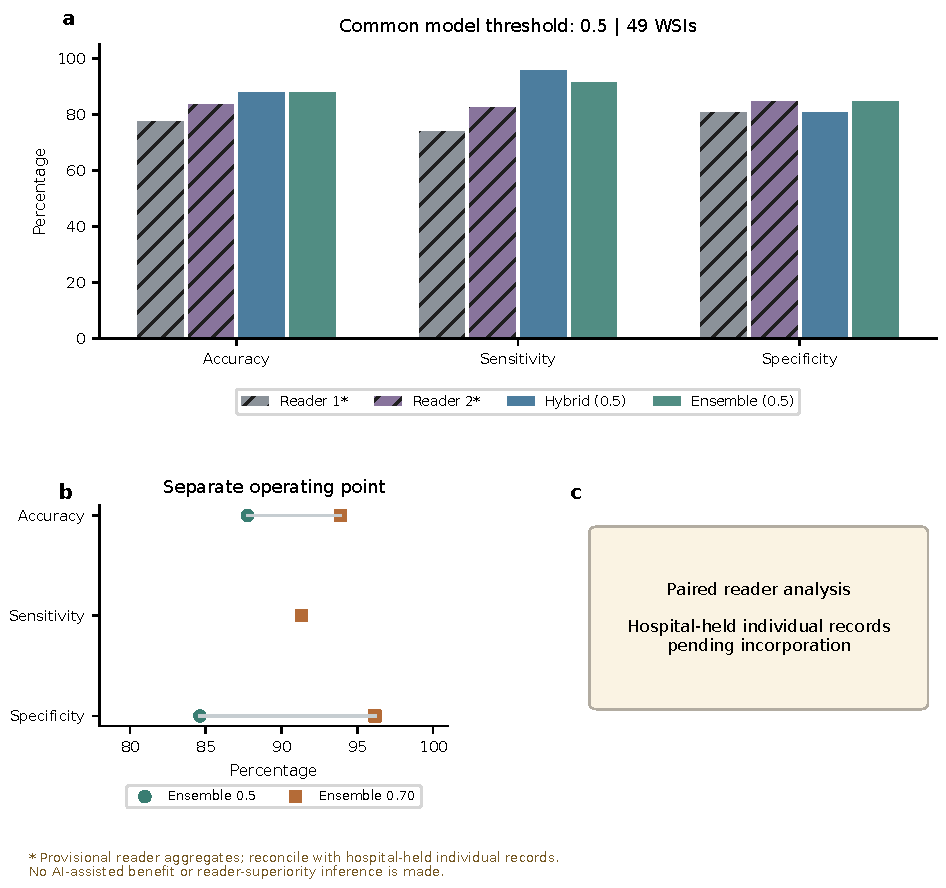
\includegraphics[width=\textwidth,height=.76\textheight,keepaspectratio]{figures/Figure_4_reader_comparison.pdf}
\caption{\textbf{Reader comparison and separate model operating points}. \textbf{a,} Provisional reader aggregates (hatched) and both models at threshold 0.5 on the 49-slide internal set. \textbf{b,} The ensemble at 0.5 and the retrospectively selected 0.70 operating point. \textbf{c,} Paired reader analyses remain unfilled pending incorporation of hospital-held records. Reader values are not assigned error bars or significance claims before reconciliation. Model estimates reuse validation slides involved in selection; no superiority inference is made. Source data are provided in reader\_aggregate\_PROVISIONAL.csv, internal\_model\_metrics.csv and ensemble\_threshold\_0\_70.json. \missing{[MISSING R01/R02: hospital-held individual reader records and subsequent paired analysis.] }}\label{fig:4}
\end{figure}
}

\newcommand{\MainFigureFive}{%
\begin{figure}[!htbp]\centering
\fbox{\begin{minipage}[c][35mm][c]{.88\textwidth}\centering
\textbf{Omitted from this public repository copy}\\[6pt]
This figure contains tissue images or individual-slide observations.\\
The complete figure is retained in the local manuscript archive.
\end{minipage}}
\caption{\textbf{Model-selected regions and internal coefficients in correct and incorrect classifications}. \textbf{a--d,} Cases 1, 4, 7 and 10 represent a true positive, true negative, false positive and false negative, respectively. Both main-evaluation and interpretation-run uncalibrated scores are shown. Overlays encode prototype margin, not attention; colors show margin divided by a per-slide scale, with saturation beyond $\pm1$. Colors encode the difference between latent-bank similarities and have no independently established disease-specific morphological meaning. Color intensity is not directly comparable between cases. H/L locators identify the highest/lowest-margin thumbnails, verified by exact pixel matching to the original sampled windows. Scale bars, 50 $\mu\mathrm{m}$; source windows span approximately 231.1 $\mu\mathrm{m}$. \textbf{e,} Gate coefficients scale feature vectors and do not establish causal importance. All eight original thumbnails, including the low-margin crop in Case 10, are retained. Archived segmentation-contour coverage is summarized in Supplementary Table S12; it does not establish pathology-confirmed tissue or lesion content. Case 10 locators preserve the historical overlay extent documented in that table. Source data include interpretation\_probability\_comparison.csv and interpretation\_gate\_weights.csv. \missing{[MISSING P03: pathology-confirmed regional descriptions.] }}\label{fig:5}
\end{figure}
}

\newcommand{\MainFigureSix}{%
\begin{figure}[!htb]\centering
\fbox{\begin{minipage}[c][35mm][c]{.88\textwidth}\centering
\textbf{Omitted from this public repository copy}\\[6pt]
This figure contains tissue images or individual-slide observations.\\
The complete figure is retained in the local manuscript archive.
\end{minipage}}
\caption{\textbf{Fixed-checkpoint sampling variability and ensemble error exchange}. \textbf{a,} Sample standard deviation of the uncalibrated Hybrid score across 20 additional 512-patch bags for each of 49 internal and 168 external WSIs; each dot is one WSI and horizontal marks denote medians. \textbf{b,} AUROC for each complete-cohort draw (20 dots per cohort). Horizontal marks denote draw medians; open diamonds denote the historical reference-bag AUROC. The spread across draws describes sampling variability, not a confidence interval. \textbf{c,} WSIs with at least one score below 0.5 and at least one score at or above 0.5 across the 20 bags, stratified by cohort and class. Labels give numerator/denominator. \textbf{d,} Correctness of archived Hybrid and ensemble predictions at threshold 0.5 on the same 49 internal WSIs. The ensemble corrects one SS error and introduces one MALT error, with five shared errors. Sampling repeats do not constitute new WSIs or retraining replicates. Source data: repeated\_bag\_predictions.csv and the archived model-specific internal predictions.}\label{fig:6}
\end{figure}
}

